%!TEX root = ../thesis.tex
% Introduction

\chapter{Fundamentos conceptuales} % (fold)
\label{cha:fundamentos_conceptuales}
	En este capítulo se presentan los elementos que permiten realizar una presentación con \textit{Beampress}. Estos elementos son \textit{Frame}, \textit{Slide Item} y \textit{Overlay}, inspirados en sus equivalentes de la clase \textit{Beamer} de \LaTeX{} y que se describen en las definiciones \ref{def:frame}, \ref{def:slide_item} y \ref{def:overlay} respectivamante. También se muestran los fundamentos de \textit{Beampressk}, básicamente su concepción como \textit{Api Rest}, para eliminar las dificultades del presentador con respecto a la distancia vistas en la sección \ref{sec:proyecto_delta}, así como la opción que brinda para usar un \textit{Live Feed}. Estos dos últimos elementos serán ampliados en las secciones \ref{sec:api_rest} y \ref{sec:live_feed} respectivamante. 

	\section{Definiciones de Beampress} % (fold)
	\label{sec:definiciones_de_beampress}
		Para dar respuesta a los requerimientos que se plantearon en la sección \ref{sec:requerimientos_basicos_del_sistema_propuesto}, se ofrecen algunas definiciones pertinentes.
		
 		\begin{definition}
 		\label{def:presentation}
			Una \textbf{presentación} es un conjunto de frames, que serán mostrados según su orden. En la fig \ref{fig:frames} se expone una presentación compuesta por tres frames.
 		\end{definition}

 		\begin{figure}[tb]
 			\centering
 			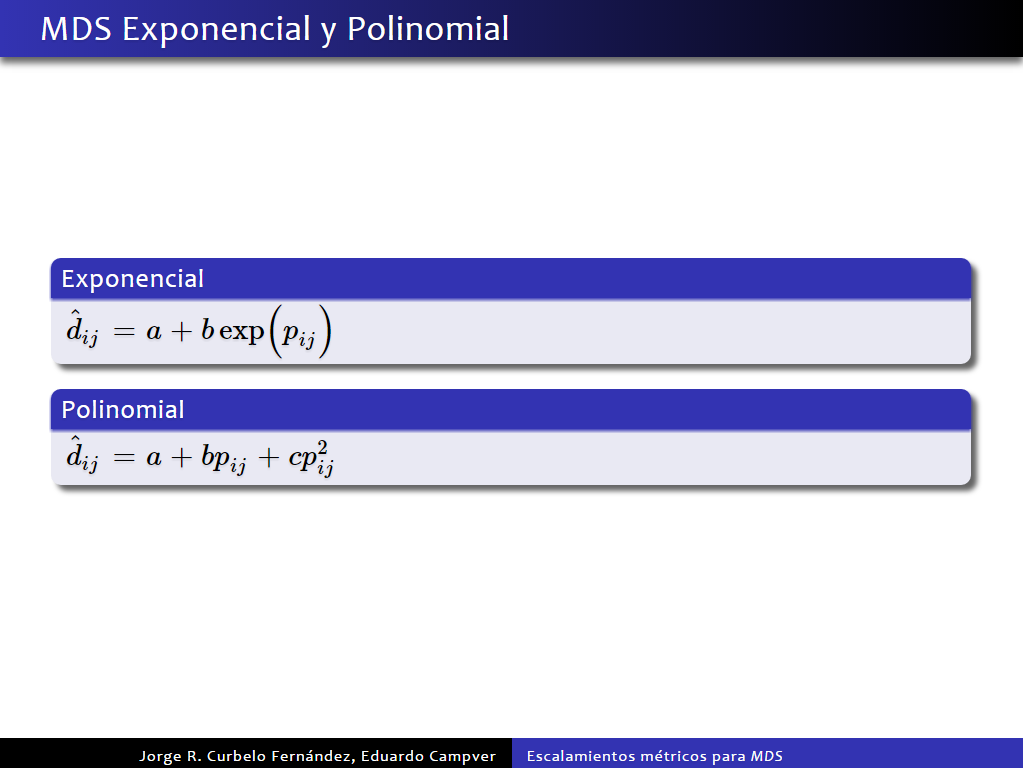
\includegraphics[width=4cm]{img/f1}
 			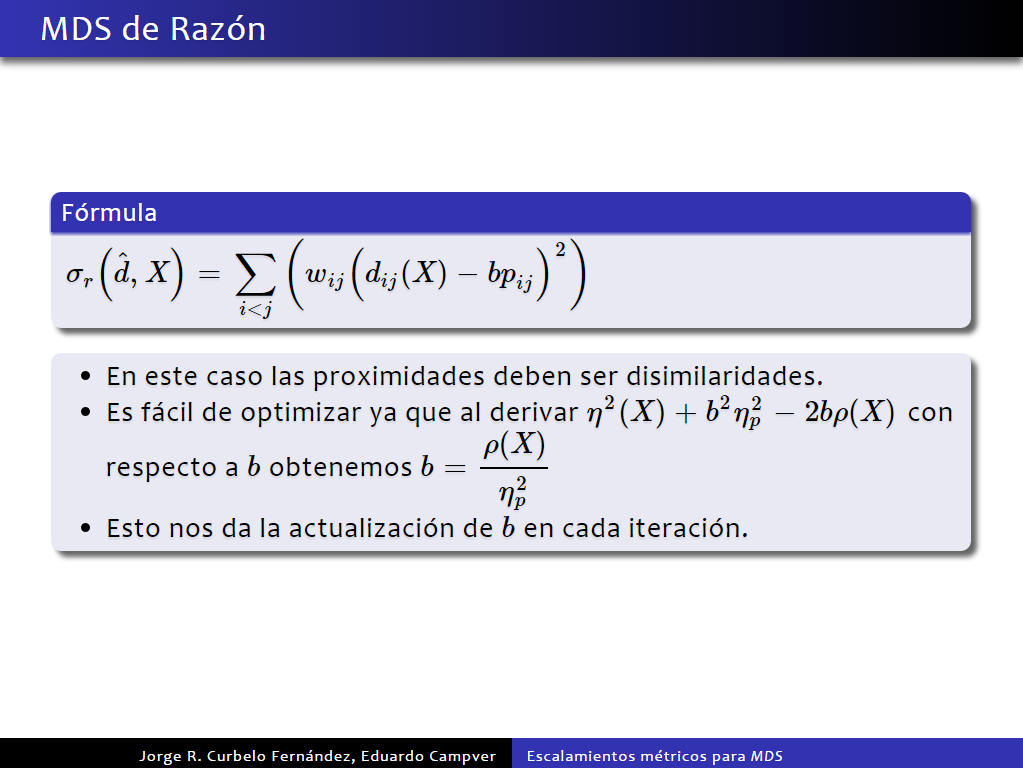
\includegraphics[width=4cm]{img/f2}
 			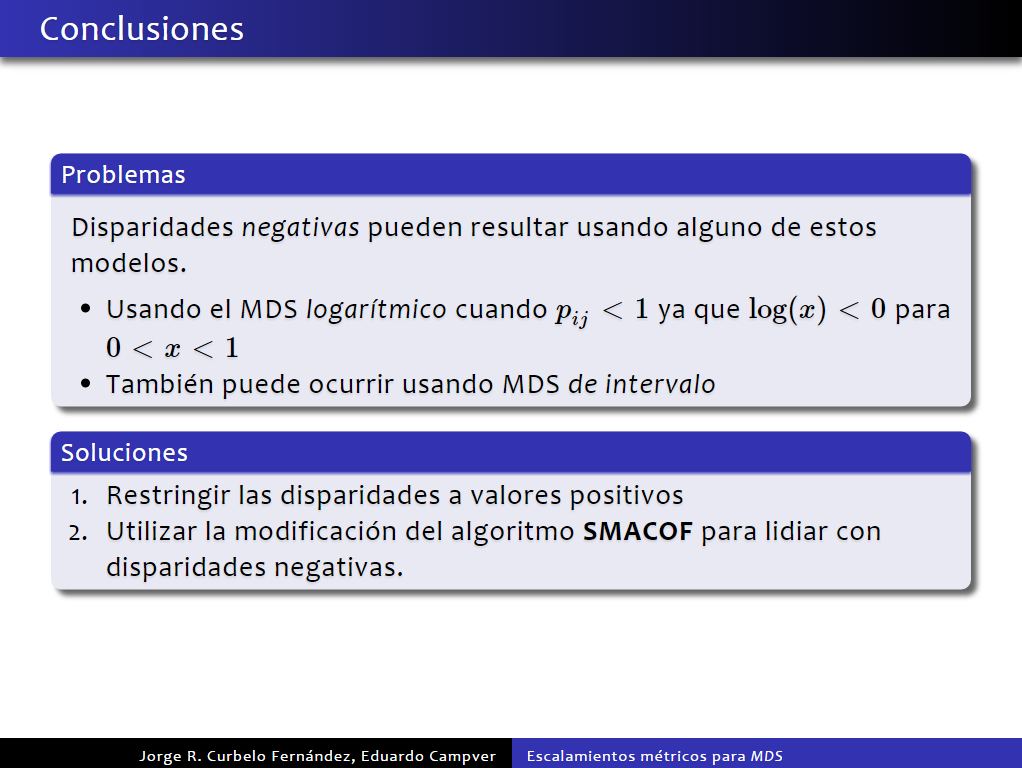
\includegraphics[width=4cm]{img/f3}
 			\caption{Ejemplo de tres frames}
 			\label{fig:frames}
 		\end{figure}

 		\begin{definition}
 		\label{def:frame}
			Un \textbf{frame} es un conjunto de \textbf{slides items} y representa una diapostiva en la presentación. Nótese que esta definición es distinta en \textit{Beamer}, donde un \textit{Frame} no es una diapositiva, sino un conjunto de ellas, mostradas de forma tal que simulen una animación.
 		\end{definition}		

		\begin{definition}
		\label{def:content}
			Un \textbf{contenido} es todo aquello que se muestre en las diapositivas, ya sea texto, imagen, audio, video o sus combinaciones posibles. En la fig \ref{fig:frame_video_image} se muestra un frame con varios contenidos: un video en la esquina superior izquierda, una imagen a su derecha y debajo tres bloques con texto.
		\end{definition}
 		\begin{figure}[tb]
 			\centering
 			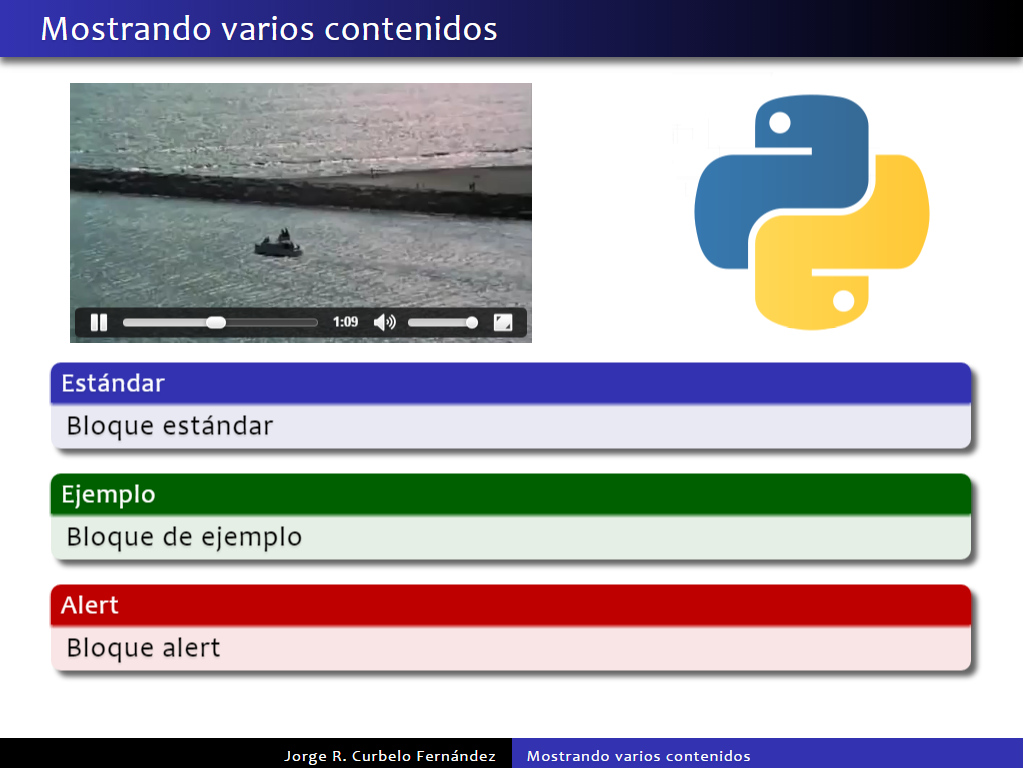
\includegraphics[width=12cm]{img/frame-video-image}
 			\caption{Ejemplo de un frame con contenidos}
 			\label{fig:frame_video_image}
 		\end{figure} 		

		\begin{definition}
		\label{def:show}
			\textbf{Mostrar} un contenido es la exhibición de imagen o de texto, la reproducción de audio o de video o cualquier combinación de estas posibilidades.
		\end{definition} 		

		Una \textit{presentación} tiene una ordenación en las diapositivas y en los \textit{contenidos}. Por ejemplo, en la fig. \ref{fig:contents} se muestra un \textit{frame} con tres \textit{contenidos} que se ven en momentos distintos. A continuación se argumentarán algunas definiciones que se tuvieron en cuenta para especificar dicha ordenación.

 		\begin{figure}[tb]
 			\centering
 			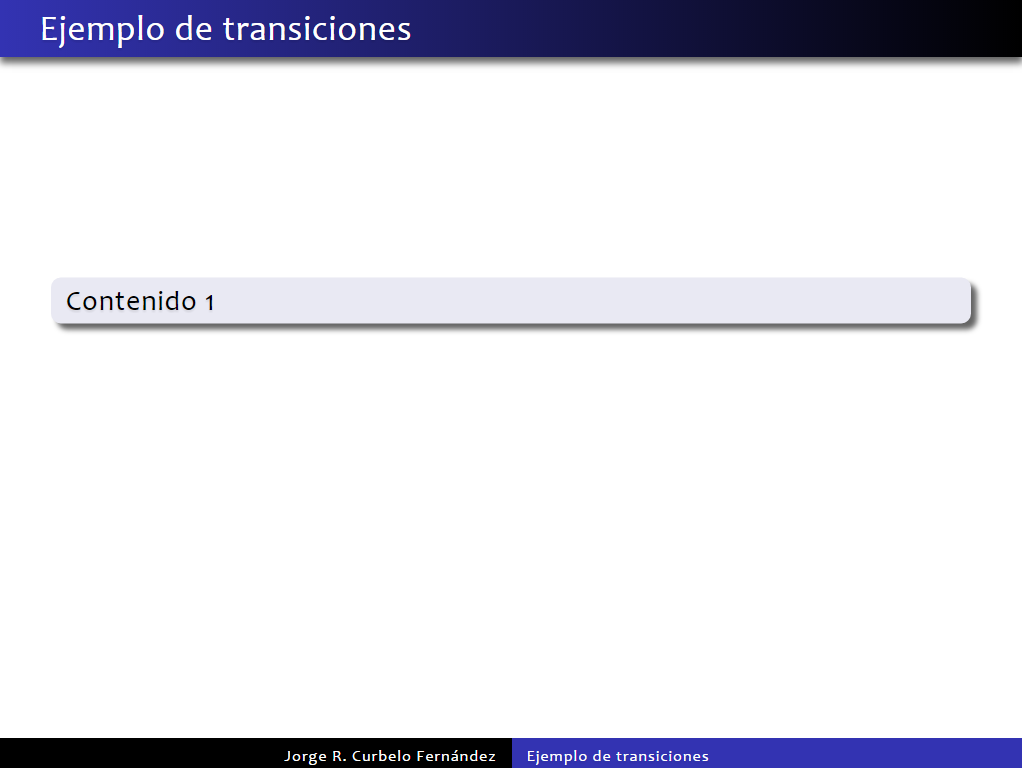
\includegraphics[width=4cm]{img/content1}
 			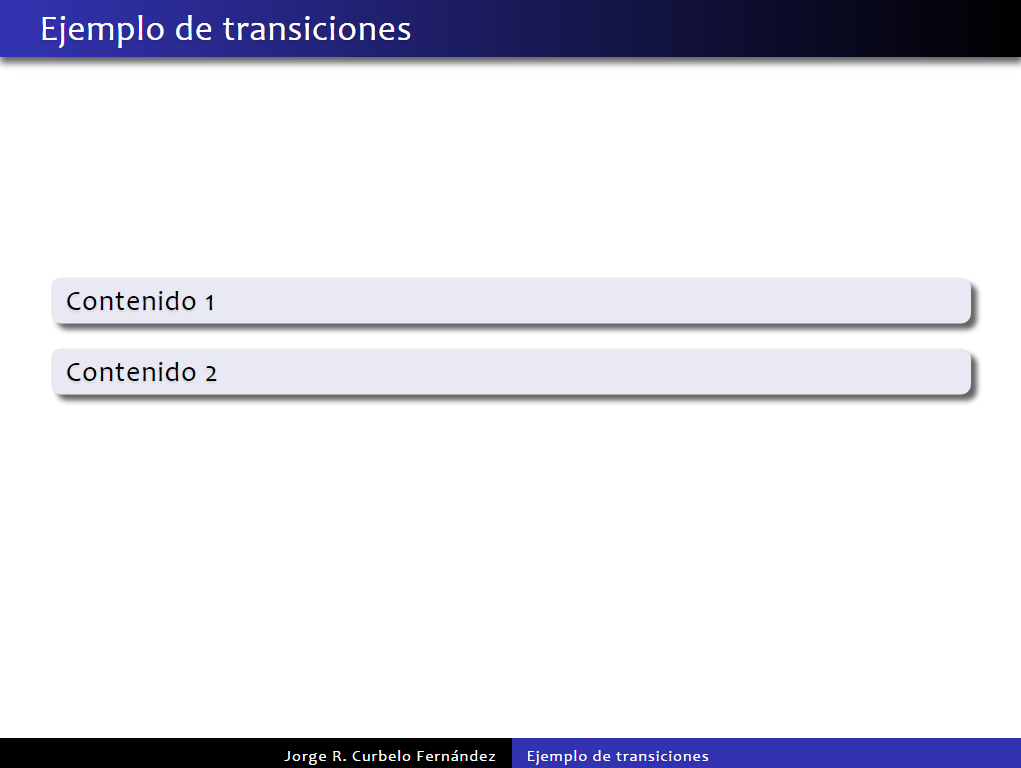
\includegraphics[width=4cm]{img/content2}
 			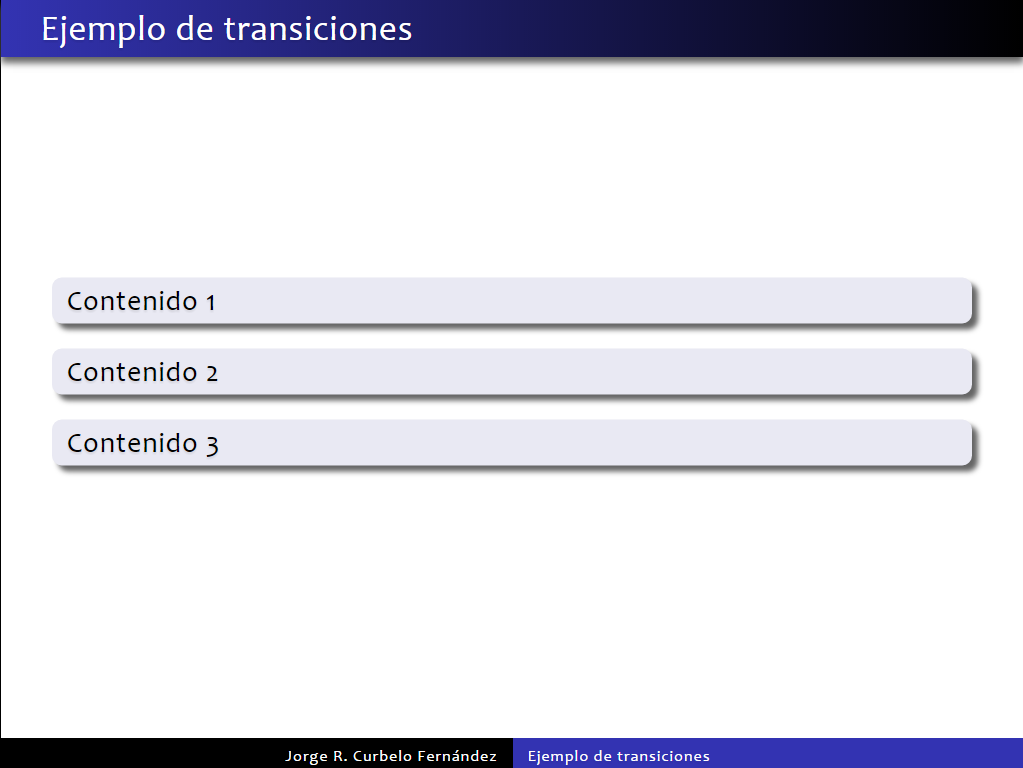
\includegraphics[width=4cm]{img/content3}
 			\caption{Ejemplo de un \textbf{frame} con tres contenidos mostrados en distintos \textbf{overlays}}
 			\label{fig:contents} 
 		\end{figure}		

 		\begin{definition}
 		\label{def:overlay}
 			Un \textbf{overlay} es un intervalo que determina un orden para mostrar un contenido. Un intervalo puede ser un número ej: 3 o bien, un rango ej: 3-5. Los límites superiores e inferiores son opcionales, pero en caso de no especificarse, para el inferior se asume 1 y para el superior se asume el último \textit{overlay} del \textit{Frame}.
 		\end{definition}

 		\begin{definition}
 		\label{def:ovaerlay_set}
 			Un conjunto de \textbf{overlays} es una lista de ninguno o varios intervalos separados por punto y coma (;). En la fig \ref{fig:overlay_set} se expone un ejemplo de cómo se define un conjunto de \textit{overlays}.
 		\end{definition} 

 		\begin{definition}
 		\label{def:slide_item}
 			Un \textbf{slide item}, es la base de los \textbf{frames}. Es un \textbf{contenido} que tiene definido un conjunto de \textbf{overlays}. Por convenio, los \textit{slide items} están \textbf{mostrados}, o sea, independientemente del \textbf{overlay} actual, se muestran si no se les especifican intervalos. Un ejemplo de \textit{slide item} puede ser la imagen del \textit{frame} en la fig \ref{fig:frame_video_image}, sin \textit{overlays}.
 		\end{definition}

		\begin{figure}[htb]%
			\centering
			$$-2; 4; 6-8; 10-$$
			\caption{Ejemplo de un conjunto de \textit{overlays}} 
			\label{fig:overlay_set}
			\small

		Para un mejor entendimiento de los conceptos ``\textit{overlay}'' y ``\textit{slide item}'' se empleará un ejemplo. Un \textit{slide item} con los intervalos de esta figura, indica que su \textit{contenido} estará \textit{mostrado} hasta el slide dos, no se \textit{mostrará} en el tres, aparecerá en el cuatro, luego en el cinco se dejará de ver, reaparecerá desde el seis hasta el ocho, en el nueve se dejará de ver y estará \textit{mostrado} desde el diez hasta el final. 			
		\end{figure}

 		\begin{definition}
 		\label{def:slide}
 			Un \textbf{slide} es un conjunto de \textbf{slide items} que se muestran simultáneamente en un \textbf{frame} dado un \textbf{overlay}.
 		\end{definition}

 		\begin{definition}
 		\label{def:transition}
 			Una \textbf{transición} es un cambio de \textbf{slide} o bien un cambio entre \textbf{frames}.
 		\end{definition}

 		\begin{definition}
 		\label{def:next_transition}
 			Una \textbf{transición siguiente} es el paso de un intervalo (\textbf{overlay}) menor a uno mayor.
 		\end{definition} 		

 		\begin{definition}
 		\label{def:prev_transition}
 			Una \textbf{transición anterior} es el paso de un intervalo (\textbf{overlay}) mayor a uno menor.
 		\end{definition}

		Para hacer uso de las \textit{transiciones} con los \textit{overlays} se explican algunas definiciones que se tomaron en cuenta.

		\begin{definition}
		\label{def:transition_func}
			Una \textbf{función de transición} en un \textbf{slide item} es el cambio de estado del \textbf{contenido} del \textbf{slide item} al ocurrir una \textbf{transición}.
		\end{definition}

		\begin{definition}
		\label{def:next_transition_func}
			Una \textbf{función de transición siguiente} en un \textbf{slide item} es el cambio de estado del \textbf{contenido} del \textbf{slide item} al ocurrir una \textbf{transición siguiente}.
		\end{definition}

		\begin{definition}
		\label{def:prev_transition_func}
			Una \textbf{función de transición anterior} en un \textbf{slide item} es el cambio de estado del \textbf{contenido} del \textbf{slide item} al ocurrir una \textbf{transición anterior}.
		\end{definition}

		Por defecto, se definen tres \textbf{funciones de transición} básicas que son las siguientes:
		\begin{itemize}
			\item \textbf{Función identidad}: No cambia el estado del \textit{contenido} del \textit{slide item}
			\item \textbf{Función mostrar}: \textit{Visualiza} el \textit{contenido} del \textit{slide item}. Esta función no cumple totalmente con la definición \ref{def:show} de \textbf{mostrar} que se argumentó, no reproduce ni audios ni videos. La capacidad de hacer uso de elementos multimedias se argumenta en la sección \ref{sec:sintaxis_extendida} 
			\item \textbf{Función ocultar}: \textit{Oculta} el \textit{contenido} del \textit{slide item}
		\end{itemize}

		Como se vió en la definición \ref{def:slide_item}, un \textbf{slide item} está \textbf{mostrado} por defecto en todos los \textbf{slides} a no ser que su \textbf{conjunto de overlays} especifique otra cosa. Luego de definir las funciones elementales, esto se traduce a que todas las \textbf{funciones de transición} de un \textbf{slide item} por defecto son la \textbf{función identidad} excepto la primera, que es la \textbf{función mostrar}. 

		\comment{A continuación se define de una forma más detallada lo antes expuesto:}{Creo que lo que viene no queda muy claro, pero para definiciones matemáticas debería preguntar primero no? Bueno, a lo mejor nada de nada queda claro}

 		Sean \( I \) y \( M \) la \textbf{función identidad} y la \textbf{función mostrar} respectivamente


        Sea \( S_j \) un \textbf{slide item}

        Entonces la \textbf{función de transición} \( f_i \) de \( S_j \) para los intervalos \( 1 \dots n \) se define de la siguiente manera:
        \comment{
		\begin{equation}
			f_i = 
			\begin{cases}
				M & \mbox{si } i = 1 \\
				I & \mbox{si } i > 1.
			\end{cases}
		\end{equation}}{No me salió bien la fórmula, el cambio de línea para los \textit{cases} is not pinching}

		A contiunación se muestra otra definición de \textbf{overlay} usando las \textbf{funciones elementales}.

		\begin{definition}
		\label{def:new_overlay}

 			Un \textbf{overlay} es un intervalo que tiene definido una \textbf{función de transición siguiente} y una \textbf{función de transición anterior}.

		\end{definition}		


	% section definiciones (end)



	Luego de señalar las concepciones de \textit{Beampress}, se resalta su similitud con \textit{Beamer} en cuanto a \textit{Overlays} y \textit{Frames}. Sin embargo, con la sintaxis para definir conjuntos de \textit{overlays} vista en la fig. \ref{fig:overlay_set} existe un problema: no es posible el uso de otras	\textbf{funciones de transición} que no sean las elementales. Con estas \textbf{funciones elementales} no se puede incluir la reproducción de audios y videos ni el uso de animaciones, requisitos para \textit{Beampress} vistos en la sección \ref{sec:requerimientos_basicos_del_sistema_propuesto}.	Por lo tanto conviene \textit{extender} o \textit{mejorar} la forma de definir los conjuntos de \textbf{overlays}.



	\section{Sintaxis extendida} % (fold)
	\label{sec:sintaxis_extendida}
	

	Teniendo en cuenta los conceptos de \textbf{slide item}, \textbf{overlay}, \textbf{conjunto de overlays} y \textbf{función de transición} vistos en las definiciones \ref{def:frame}, \ref{def:overlay}, \ref{def:ovaerlay_set} y \ref{def:transition_func} respectivamente, se propone a continuación definir una extensión a la sintaxis vista en la fig.\ref{fig:overlay_set}. Como ejemplo, se muestra en la fig. \ref{fig:json_format} una alternativa para definir \textit{overlays} con cualquier \textit{función de transición}.

		\begin{figure}[htb]%
			\begin{lstlisting}%

'{"número":{"siguiente":{"func":"nombre-de-función", "args":{...}}, "anterior": {"func":"nombre-de-función", "args":{...}}}}'	
			\end{lstlisting}
		\caption{
			Formato JSON para un \textbf{overlay} con funciones de transición. 
			\label{fig:json_format} }
		\end{figure}


	En este caso, un intervalo puede ser un JSON con las siguientes características:
	\begin{itemize}
		\item ``número'' es el número del intervalo
		\item ``next'' tiene como valores, el nombre de la \textbf{función de transición siguiente} a utilizar y sus argumentos
		\item ``prev'' es lo mismo que ``next'' pero recibe el nombre de la \textbf{función de transición anterior}
	\end{itemize}

	Una de las principales motivaciones para la creación de \textit{Beampress} fue el requerimiento de animaciones, audio y video vistas en la sección \ref{sec:requerimientos_basicos_del_sistema_propuesto}, para lo cual resulta imprescindible el manejo de dicha sintaxis transformada. Por ejemplo, si se quiere reproducir un audio o un video podemos se puede utilizar lo que se muestra en la fig. \ref{fig:ex_audio_video_syntax}.
	\begin{figure}[htb]%
		\begin{lstlisting}%


'{"1":{"next":{"func":"fadeInVideo", "args":{"currentTime": "30"}}, "prev": {"func":"fadeOutVideo", "args":{}}}}'
'{"2":{"next":{"func":"fadeInAudio", "args":{"currentTime": "10"}}, "prev": {"func":"fadeOutAudio", "args":{}}}}'  
				
		\end{lstlisting}
		\caption{Ejemplo de uso de audio y sonido} 
			\label{fig:ex_audio_video_syntax}
		\small Se hará un \textit{fade in} para reproducir el video en el \textit{overlay} 1 comenzando en el segundo 30. Lo mismo sucederá con el audio, pero en el \textit{overlay} 2 y comenzando en el segundo 10.
		\end{figure}

		La utilización de esta sintaxis permite el empleo de \textit{cualquier} \textbf{función de transición} que se defina, en la sección \ref{cha:extensibilidad} se hablará de esta característica con más detalles. Un ejemplo de un \textbf{overlay} con una \textbf{función de transición} distinta de las funciones elementales, se puede apreciar en la fig. \ref{fig:ball_code} y su ejemplo visual en la fig. \ref{fig:ball_visual}.



		\begin{figure}[htb]%
			\begin{lstlisting}%

'{"3": {
    "next": {
        "func": "rollBallToLeft",
        "args": {}
    },
    "prev": {
        "func": "rollBallToRight",
        "args": {}
    }
}}''
			\end{lstlisting}
		\caption{Ejemplo del empleo de una \textbf{función de transición} en un \textbf{overlay}} 
			\label{fig:ball_code} }
		\end{figure}	




 		\begin{figure}[tb]
 			\centering
 			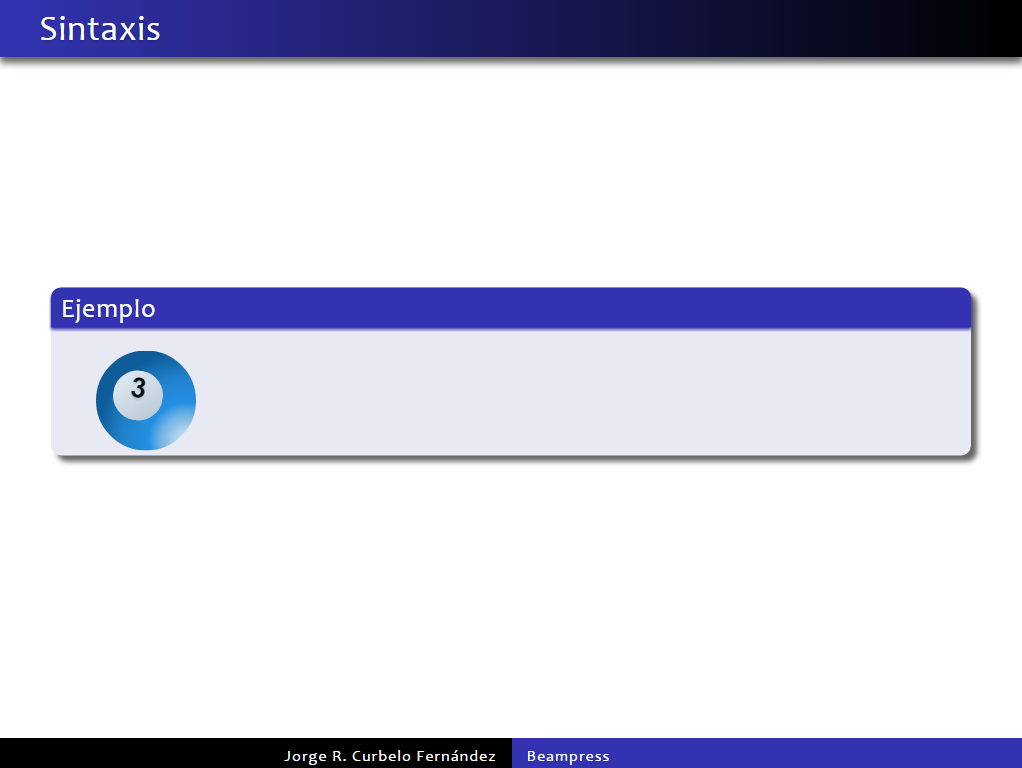
\includegraphics[width=4cm]{img/ball-left}
 			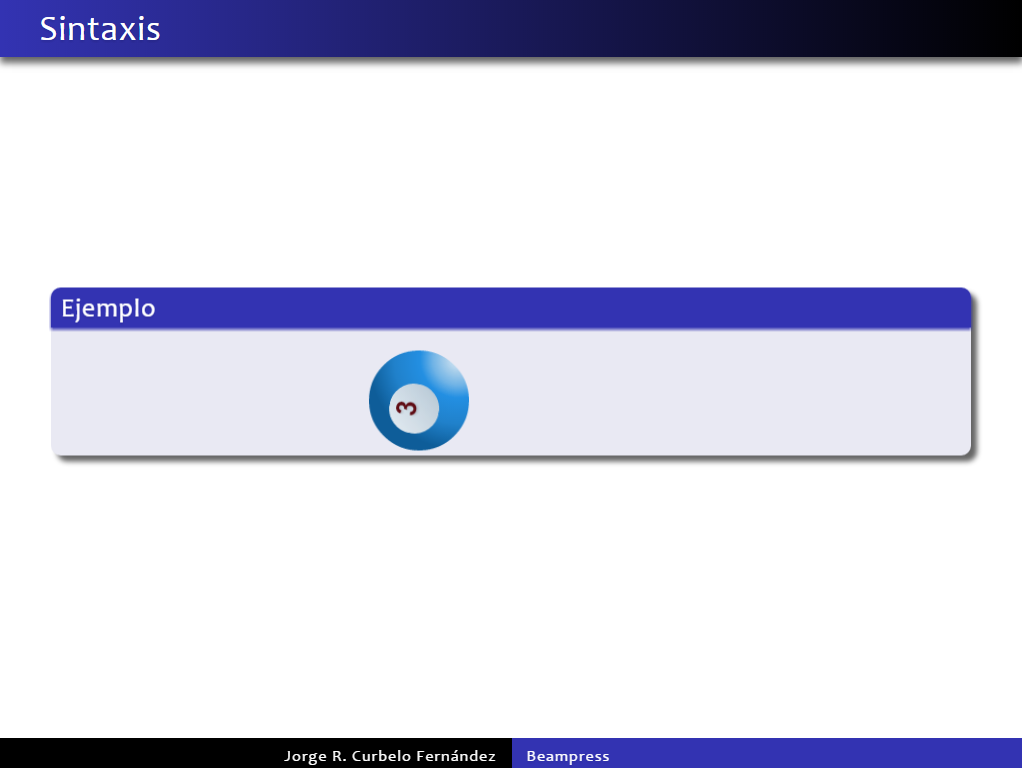
\includegraphics[width=4cm]{img/ball-middle}
 			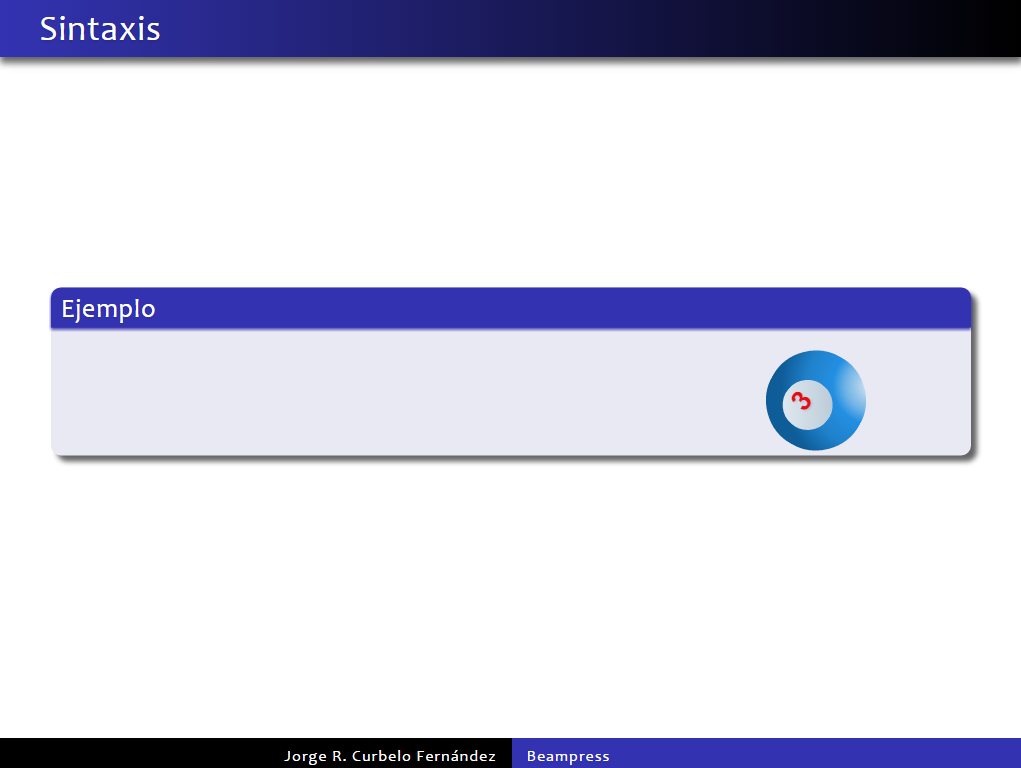
\includegraphics[width=4cm]{img/ball-right}
 			\caption{Ejemplo visual del \textbf{overlay} definido en la fig. \ref{fig:ball_code}}
 			\label{fig:ball_visual} 
 		\end{figure}	


	Dada la posibilidad de empleo de esta sintaxis, también se puede utilizar para definir las \textbf{funciones de transición} de los \textit{Frames}. En la fig. \ref{fig:frame_trans} se muestra un ejemplo de esto.

		\begin{figure}[htb]%
			\begin{lstlisting}%

'{"func":"slowShowFrame", "args":{}}'
'{"func":"slowHideFrame", "args":{}}'
			\end{lstlisting}
		\caption{
			\textbf{Funciones de transición para un frame}. 
			\label{fig:frame_trans} }
		\end{figure}	

	% section sintaxis_extendida (end)

	\section{Definiciones de Beampressk} % (fold)
	\label{sec:definiciones_de_beampressk}
	
	% section definiciones_de_beampressk (end)

	\section{Api Rest} % (fold)
	\label{sec:api_rest}
		La \textbf{Transferencia de Estado Representacional} (Representational State Transfer) o \textbf{REST} es una arquitectura simple y \textit{sin estados} que generalmante funciona a través del protocolo \textbf{HTTP}. En los últimos años \textbf{REST} ha emergido como el diseño de la arquitectura estándar para servicios web (Servicios RESTful) y APIs web.

		Conjuntamente con el concepto de un servicio RESTful está la noción de \textit{recursos}. Los recursos son representados por URIs, un cliente envía un pedido (request) a estas URIs usando los métodos definidos por el protocolo \textbf{HTTP}, y posiblemente el estado de dicho recurso cambie como resultado de dicho pedido.

		Los pedidos HTTP son diseñados para afectar un recurso en diversas formas:

		\begin{table}[tb]
			\caption{Tipos de pedidos HTTP con sus acciones}
			\label{tab:request}
			\centering
		
			\begin{tabular}{l|c|r}
			\hline
		
			\hline
			\textbf{Método} & & \\ 
			\textbf{HTTP} & \textbf{Acción} & \textbf{Ejemplos} \\
			\hline
				GET & Obtener información &  http://beampressk.com/api/frames \\ 
				& de un recurso & (obtener una lista de frames) \\
			\hline

			\hline
				GET & Obtener información &  http://beampressk.com/api/frames/3 \\ 
				& de un recurso & (obtener el frame 3) \\
			\hline

			\hline
				POST & Crea un nuevo &  http://beampressk.com/actions/msg \\ 
				& recurso & (crea un mensaje \\ 
				& &con datos del pedido)\\
			\hline

			\hline
				DELETE & Elimina un &  http://beampressk.com/frames/delete/4 \\ 
				& recurso & (borra \\ 
				& &el frame 4)\\
			\hline										
		
			\hline
			\end{tabular}
		\end{table}
		
	% section api_rest (end)	

	\section{Extensibilidad} % (fold)
	\label{sec:extensibilidad}
	
	% section extensibilidad (end)		

% chapter fundamentos_conceptuales (end)




